\documentclass{article}
\usepackage[utf8]{vietnam}
\usepackage{mathtools}
\usepackage{amssymb}
\usepackage[a4paper, total={6in, 8in}]{geometry}
\usepackage{graphicx}
\usepackage{tikz}
\usetikzlibrary{calc}
\usepackage[skip=10pt plus1pt, indent=20pt]{parskip}
\usepackage{indentfirst}
\usepackage{float}
\usepackage{caption}
\usepackage{listings}
\usepackage{xcolor}

\definecolor{codegreen}{rgb}{0,0.6,0}
\definecolor{codegray}{rgb}{0.5,0.5,0.5}
\definecolor{codepurple}{rgb}{0.58,0,0.82}
\definecolor{backcolour}{rgb}{0.95,0.95,0.92}

\lstdefinestyle{mystyle}{
    backgroundcolor=\color{backcolour},   
    commentstyle=\color{codegreen},
    keywordstyle=\color{magenta},
    numberstyle=\tiny\color{codegray},
    stringstyle=\color{codepurple},
    basicstyle=\ttfamily\footnotesize,
    breakatwhitespace=false,         
    breaklines=true,                 
    captionpos=b,                    
    keepspaces=true,                 
    numbers=left,                    
    numbersep=5pt,                  
    showspaces=false,                
    showstringspaces=false,
    showtabs=false,                  
    tabsize=2
}

\lstset{style=mystyle}
\usepackage{subcaption}
\newcommand\HRule{\rule{\textwidth}{1pt}}

\begin{document}
\begin{titlepage}

\begin{tikzpicture}[remember picture, overlay]
  \draw[line width = 4pt] ($(current page.north west) + (0.5in,-0.5in)$) rectangle ($(current page.south east) + (-0.5in,0.5in)$);
\end{tikzpicture}

\begin{center}
% Upper part of the page
{
\textsc{\Large Học viện Kỹ thuật Mật mã}\\
\textsc{\Large Khoa Công nghệ thông tin}\\
\HRule \\[0.4cm]
\begin{figure}[h]
\centering
\includegraphics[width=0.4\textwidth]{logo-hvktmm.png}
\label{school-logo}
\end{figure}
% Title
\HRule \\[0.4cm]
\textsc{\Large BẢO MẬT AN TOÀN HỆ THỐNG NHÚNG}\\[1cm]
{ \huge \bfseries Bảo mật video truyền trên mạng WiFi sử dụng Raspberry Pi và giao thức ZeroMQ
}\\[0.4cm]
\HRule \\[3cm]
\begin{minipage}{0.5\textwidth}
\begin{flushleft} \large
\emph{Sinh viên thực hiện:}\\
Trương Quốc Quân - CT030440
\\
Trần Gia Lương - CT030433
\break
\end{flushleft}
\end{minipage}
\begin{minipage}{0.45\textwidth}
\begin{flushright} \large
\emph{Người hướng dẫn:} \\
Lê Thị Hồng Vân
\break \break
\end{flushright}
\end{minipage}

\vfill

% Bottom of the page
{\large \today}
}
\end{center}
\end{titlepage}

\fontsize{12}{10}
\selectfont

\tableofcontents

\newpage

\listoffigures
\newpage

\listoftables
\newpage

\begin{center}
\textbf{\Large{LỜI CẢM ƠN}}
\end{center}

Trước tiên với tình cảm sâu sắc và chân thành nhất, cho phép chúng em được bày tỏ lòng biết ơn đến các thầy cô ở khoa Công nghệ Thông tin – Học viện Kỹ thuật Mật mã đã truyền đạt vốn kiến thức quý báu cho chúng em trong suốt thời gian học tập tại trường. Nhờ có những kiến thức mà thầy cô hướng dẫn, dạy bảo nên chuyên đề nghiên cứu của chúng em mới có thể hoàn thiện tốt đẹp.

Nhóm chúng em xin gửi lời cảm ơn sâu sắc đến cô Lê Thị Hồng Vân – người đã trực tiếp giúp đỡ, quan tâm, hướng dẫn chúng em hoàn thành tốt bài báo cáo này. Vì thời gian và kiến thức còn hạn hẹp nên bài báo cáo chuyên đề không thể tránh khỏi những thiếu sót, chúng em rất mong nhận được những ý kiến đóng góp quý báu của cô để kiến thức của chúng em trong lĩnh vực này được hoàn thiện hơn đồng thời có cơ hội học thêm được nhiều kinh nghiệm và sẽ hoàn thành tốt hơn trong các bài báo cáo sắp tới.

Chúng em xin chân thành cảm ơn!

\newpage

\begin{center}
\textbf{\Large{LỜI MỞ ĐẦU}}
\end{center}


Cùng với sự phát triển của xã hội, vấn đề an ninh, bảo mật đang được yêu cầu ngày càng khắt khe, đòi hỏi sự nghiên cứu, tìm tòi và phát triển không ngừng trong lĩnh vực Khoa học – Kĩ thuật.

Theo một bản báo cáo bởi Andrew Laughlin trên Which.co.uk, các camera an ninh sản xuất tại Thâm Quyến, Trung Quốc thường không được kiểm tra chất lượng trước khi được bán ra thị trường. Theo ước tính của một chuyên gia bảo mật tại Anh, hiện đang có 50,000 chiếc camera theo dõi đang hoạt động tại Anh, và khoảng 2 triệu camera trên toàn thế giới, không hề có các biện pháp bảo mật dữ liệu và chứa những lỗ hổng bảo mật. Các camera này là con mồi ngon cho những hacker thực hiện các hoạt động bất chính nhằm trục lợi.

Công ty Context Information đã thực hiện kiểm thử xâm nhập (penetration testing) 4 camera ngẫu nhiên mua trên Amazon, và tìm ra các lỗ hổng bảo mật trên cả 4 chiếc. Các lỗ hổng bảo mật có mức độ từ trung bình đến nghiêm trọng: Vstarcam C7837WIP có mật khẩu ban đầu kém; ieGeek 1080p và Sricam 720p gửi thông tin không mã hóa qua mạng Internet, Victure 1080p cho phép hacker nhận quyền root, điều khiển các thiết bị IoT khác trong hệ thống.

Có thể thấy rằng, vấn đề an toàn và bảo mật trên hệ thống nhúng đang rất nhức nhối, cần được giải quyết chặt chẽ, để bảo vệ tính riêng tư của người dùng cuối.

Trong bài báo cáo môn học này, chúng em tìm hiểu quá trình mã hóa tín hiệu video bằng thuật toán AES trước khi truyền qua mạng Wifi, thông qua giao thức \O MQ, máy tính vi mạch Raspberry Pi 3 B+, cảm biến máy ảnh Sunny P5V04A và giao diện 15-pin kết nối cảm biến với máy tính. Về phần mềm, chúng em tìm hiểu về giao thức \O MQ (ZeroMQ) thông qua thư viện PyZMQ, thư viện OpenCV 2 - thư viện hàng đầu cho lĩnh vực thị giác máy tính, thư viện PyCryptodome dành cho mã hóa AES.

\newpage

\section{Giới thiệu chung về đề tài}
\subsection{Giới thiệu đề tài}
\subsubsection{Mục tiêu}

Mục tiêu của bài báo cáo là xây dựng được một mô hình Camera - Máy tính với mối quan hệ nhiều - nhiều (mô hình Publishers - Subscribers), với các Camera là Publishers và các Máy tính là Subscribers. Các Publishers sẽ truyền dữ liệu đã mã hóa qua đường truyền tới các Subscriber cùng mạng Wifi nhờ giao thức \O MQ.

\subsubsection{Đối tượng nghiên cứu}
Với phần cứng, chúng em tập trung tìm hiểu Raspberry Pi 3 B+ và cảm biến hình ảnh Sunny P5V04A.
\par
Với phần mềm, chúng em tập trung tìm hiểu giao thức \O MQ thông qua thư viện PyZMQ, thư viện Thị giác máy tính OpenCV 2, và thư viện mã hóa PyCryptodome.
\par
\subsubsection{Phương pháp nghiên cứu}
Phương pháp được chọn là phương pháp Top – Down. 
\par
Phương pháp này tiếp cận bài toán theo hướng xem xét bài toán từ các khía cạnh chi tiết và sau đó mới tổng quát lên. Quy trình Top – Down thường được áp dụng cho các bài toán đã có giải pháp công nghệ cả về phần mềm cũng như phần cứng. Các giải pháp này đã được phát triển trước đó ở các ứng dụng khác, và đã được kiểm định. Trong thực tế chúng ta sẽ thấy, bản chất hay mấu chốt của quy trình là vấn đề tìm hiểu và xác định bài toán, làm sao để xác định được chính xác và đầy đủ nhất các yêu cầu cũng các rằng buộc mà hệ thống phải đạt được.
\par
\subsubsection{Dự đoán kết quả }
Kết quả của bài báo cáo là một hệ thống Camera - máy tính với khả năng truyền và nhận tín hiệu hình ảnh đã mã hóa với mối quan hệ nhiều - nhiều.
\par
\subsection{Giới thiệu phần cứng}
\subsubsection{Raspberry Pi 3 B+}

\begin{figure}[ht]
\centering
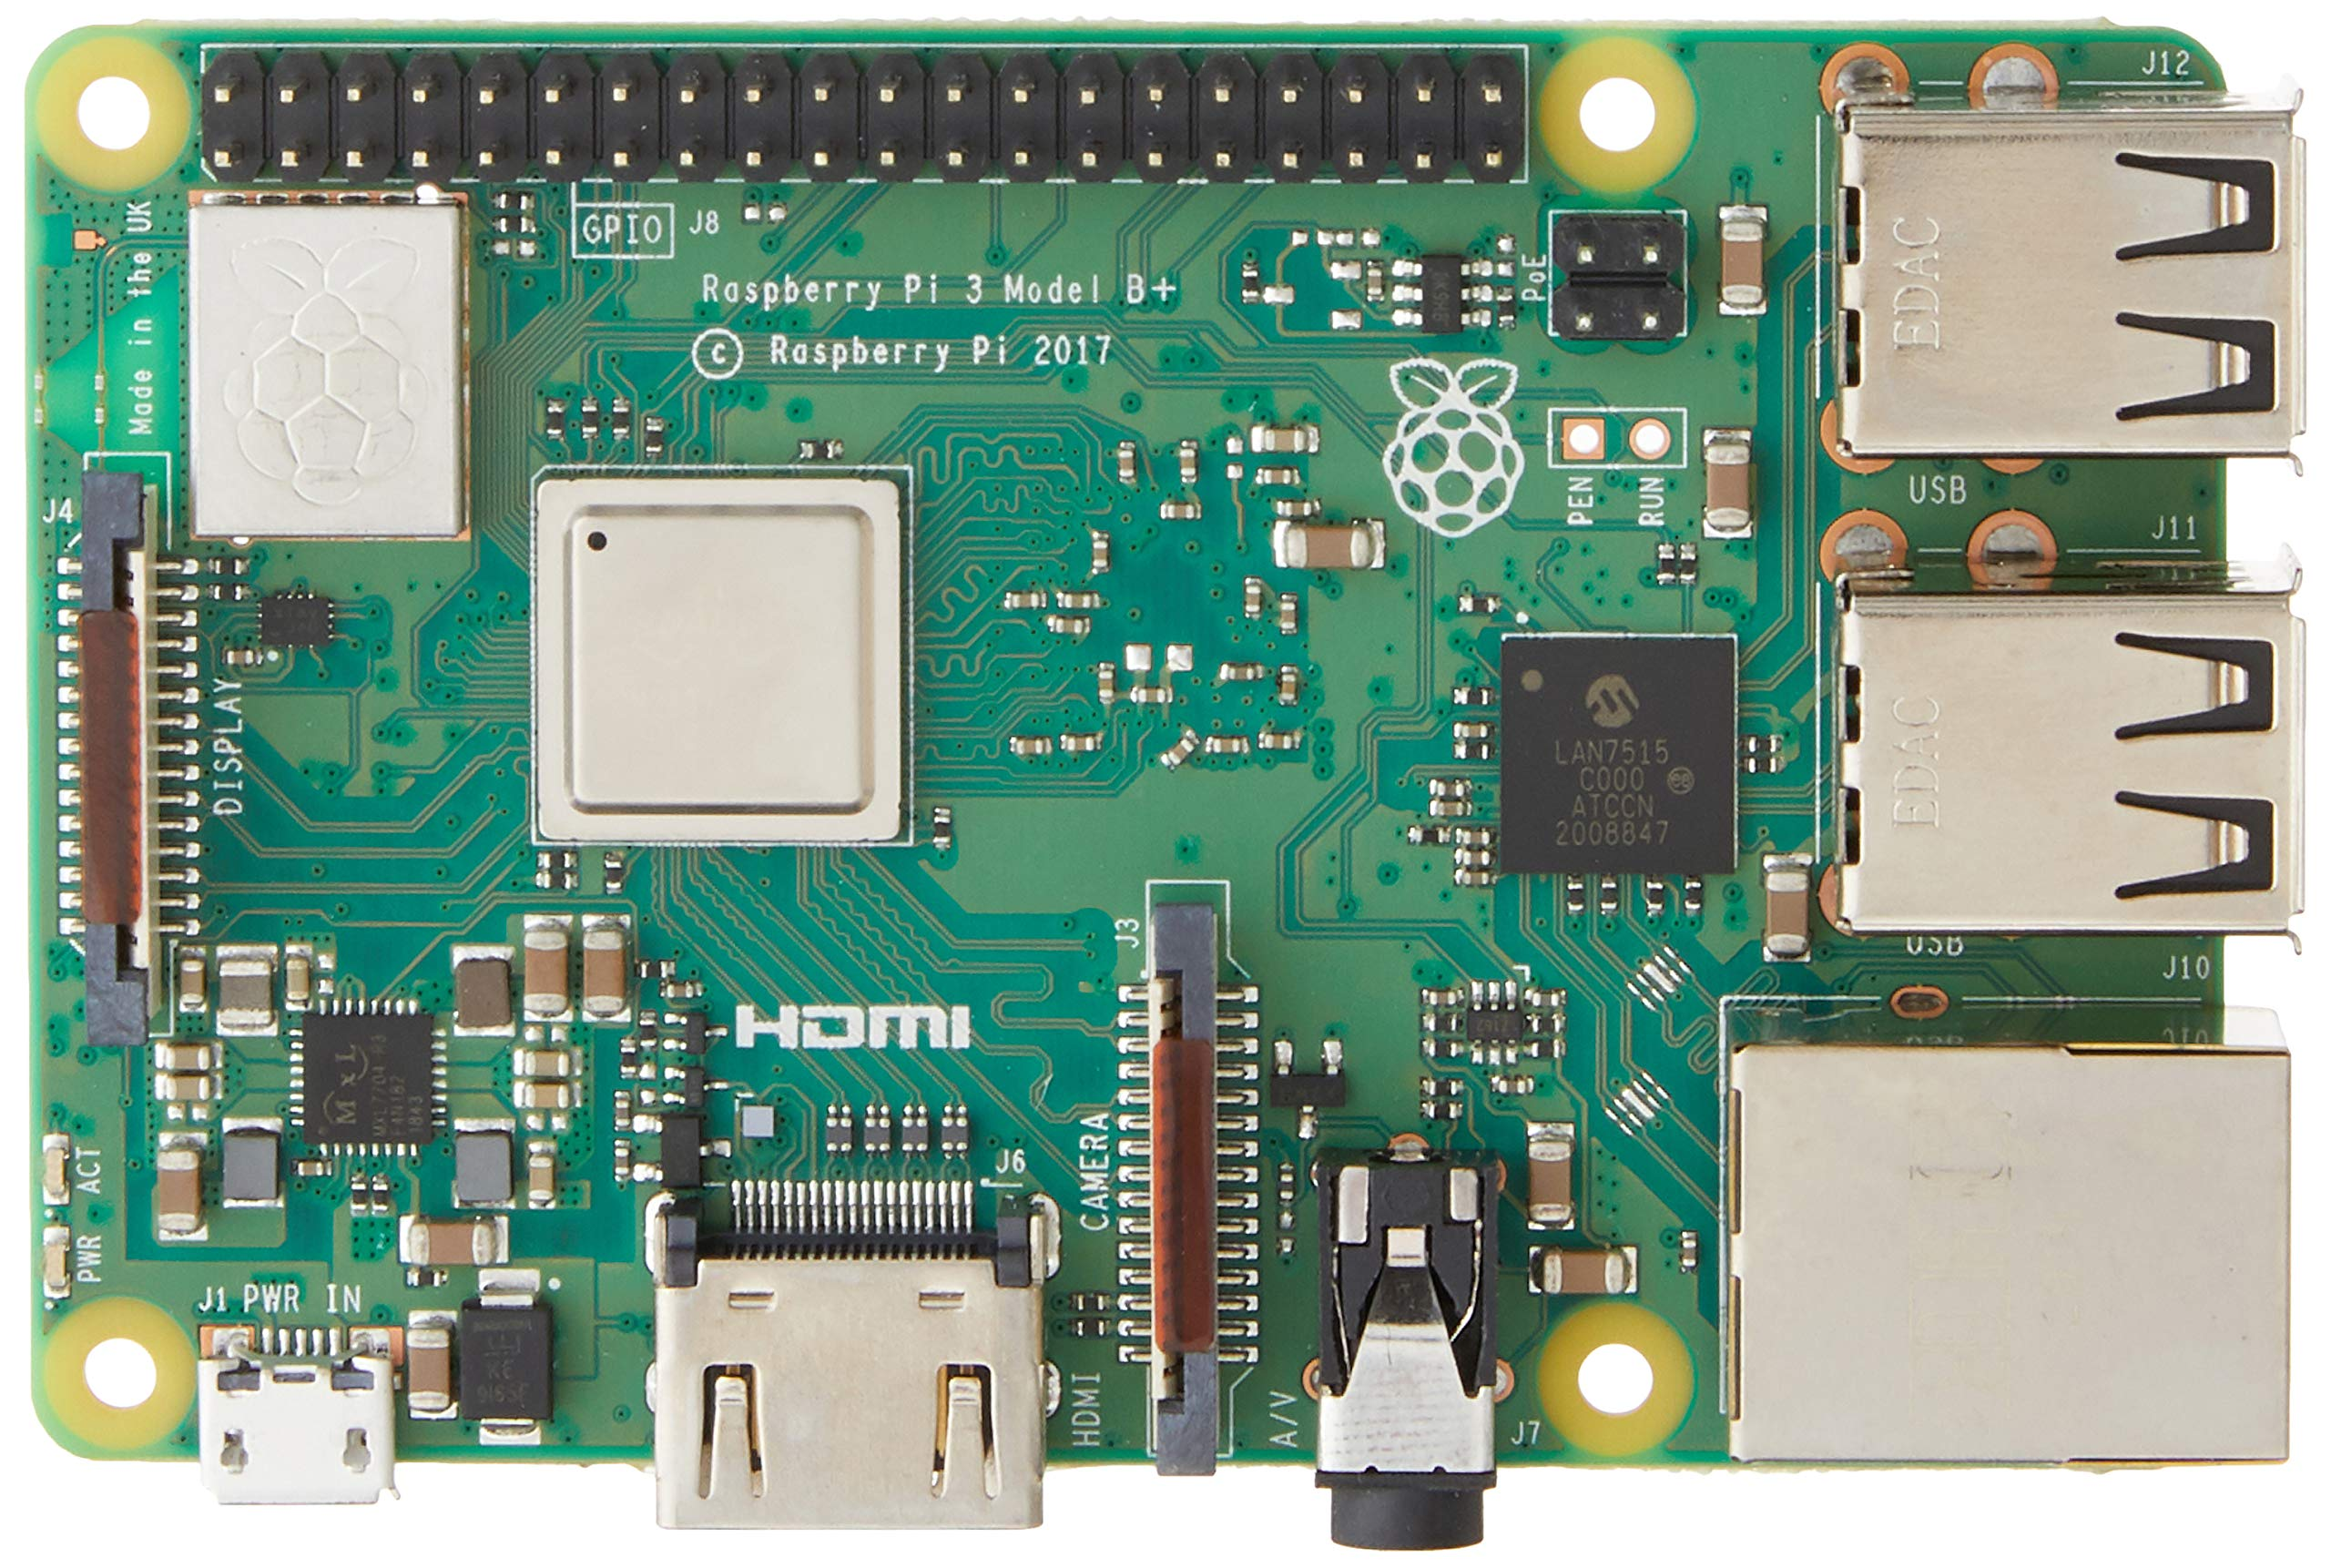
\includegraphics[width=0.6\textwidth]{rasp-pi.jpg}
\label{rasp-pi}
\caption{Raspberry Pi 3 B+}
\end{figure}

Raspberry Pi 3 là một board máy tính đơn nhỏ, giá rẻ, kích thước chỉ bằng một thẻ tín dụng, tiết kiệm điện năng (vì nguồn điện cung cấp cho RPi chỉ có 5V) được giới thiệu bởi Raspberry Pi Foundation, đi kèm với CPU, GPU, cổng USB và các chân I/O và có khả năng thực hiện một số chức năng đơn giản như một máy tính thông thường.

Máy tính nhỏ bé này được phát triển với mục đích làm cho quá trình học máy tính trở nên dễ dàng để một học sinh trung bình có thể nhận được lợi ích và dự đoán những gì một máy tính tiên tiến có thể làm.

Raspberry Pi 1 (Model B thế hệ đầu tiên) ra đời vào năm 2012 và sớm nổi tiếng về sự dễ sử dụng và tính sẵn có. Tương tự, Raspberry Pi 2 được giới thiệu vào tháng 2 năm 2015 với một chút cải tiến về thiết kế có thêm RAM so với phiên bản trước.

Được giới thiệu vào năm 2016, Raspberry Pi 3 Model B đi kèm với bộ xử lý lõi tứ cho thấy hiệu năng mạnh mẽ gấp 10 lần Raspberry Pi 1. Và tốc độ của Raspberry Pi 3 cao hơn 80\% so với Raspberry Pi 2.

Phần cứng Raspberry đã trải qua một số biến thể về hỗ trợ thiết bị ngoại vi và dung lượng bộ nhớ. Mỗi bổ sung mới đều đi kèm với một chút cải tiến về mặt thiết kế trong đó các tính năng nâng cao được thêm vào trong thiết bị để nó có thể thực hiện càng nhiều chức năng càng tốt như một máy tính thông thường.

WiFi và Bluetooth không có trong các phiên bản cũ hơn (Pi 1 và Pi 2), được thêm vào trong phần bổ sung mới của thiết bị này (Pi 3), cho phép duy trì kết nối với các thiết bị ngoại vi mà không cần sự tham gia của bất kỳ kết nối vật lý nào.

Raspberry Pi Foundation gần đây đã ra mắt Raspberry Pi 3 Model B + vào ngày 14 tháng 3 năm 2018, đây là phiên bản gần đây nhất của Raspberry Pi 3 trưng bày tất cả các thông số kỹ thuật được giới thiệu trong Pi 3 Model B, với cải tiến bổ sung bao gồm khởi động mạng, khởi động USB và nguồn qua Ethernet, điều này làm cho thiết bị trở nên hữu ích ở những nơi khó tiếp cận.

\begin{table}[ht]
    \centering
    \begin{tabular}{p{0.2\linewidth}|p{0.7\linewidth}}
    \hline
       Vi xử lý & Broadcom BCM2837B0, quad-core A53 (ARMv8) 64-bit SoC @1.4GHz \\
    \hline
       RAM  &  1GB LPDDR2 SDRAM \\
    \hline
       Kết nối  &  2.4GHz and 5GHz IEEE 802.11 b/g/n/ac wireless LAN, Bluetooth 4.2, BLE, Gigabit Ethernet over USB 2.0 (Tối đa 300Mbps) \\
    \hline
       Cổng USB  &  4 x 2.0 \\
    \hline
       Mở rộng  &  GPIO 40 chân \\
    \hline
       Video và âm thanh  &  1 cổng full-sized HDMI, Cổng MIPI DSI Display, cổng MIPI CSI Camera, cổng stereo output và composite video 4 chân \\
    \hline
       Multimedia  &  H.264, MPEG-4 decode (1080p30), H.264 encode (1080p30); OpenGL ES 1.1, 2.0 graphics \\
    \hline
       Lưu trữ  &  MicroSD \\
    \hline
       Nguồn điện  &  5V/2.5A DC cổng microUSB, 5V DC trên chân GPIO, Power over Ethernet (PoE)  (yêu cầu thêm PoE HAT) \\
    \hline
    \end{tabular}
    \caption{Thông số kỹ thuật của Raspberry Pi 3 B+}
    \label{tab:my_label}
\end{table}

\subsubsection{Cảm biến hình ảnh Sunny P5V04A}

Camera Raspberry Pi V1 Sunny P5V04A 5MP là phiên bản đầu tiên của module camera cho Raspberry Pi với cảm biến Sunny P5V04A độ phân giải 5MP, sử dụng tương thích với tất cả các dòng Raspberry Pi (Raspberry Pi Zero cần thêm cáp chuyển), chất lượng hình ảnh tốt, độ phân giải cao và có khả năng quay phim ở chất lượng HD.

\begin{figure}[ht]
\centering
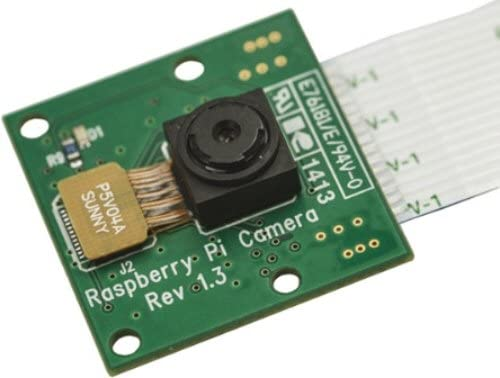
\includegraphics[width=0.6\textwidth]{Sunny.jpg}
\label{Sunny P5V04A}
\caption{Cảm biến Sunny P5V04A}
\end{figure}

Thông số kỹ thuật:
\begin{table}[ht]
    \centering
    \begin{tabular}{p{0.2\linewidth}|p{0.7\linewidth}}
    \hline
Cảm biến & Sunny P5V04A \\
\hline
Độ phân giải & 5MP \\ \hline
Góc nhìn (chéo) & 62.2 độ \\ \hline
Phân giải ảnh & 2592x1944 px. \hfill
\break
Quay phim HD 1080P 30, 720P 60, VGA 640x480P 60.\\ \hline
Lens & Fixed Focus. \\ \hline
Kết nối & Cổng kết nối 12 chân.\\
\hline
Kích thước & 25x24x9mm \\
\hline
    \end{tabular}
    \caption{Thông số kỹ thuật cảm biến hình ảnh SUNNY}
    \label{sunny}
\end{table}
\subsection{Giới thiệu thư viện}
\subsubsection{Thư viện truyền tin \O MQ}
\O MQ (còn gọi ZeroMQ) là một thư viện trao đổi gói tin không đồng bộ, nhằm mục đích sử dụng trong các app phân tán hoặc song song. \O MQ cung cấp một hàng đợi tin nhắn, nhưng khác middleware hướng thông điệp,  hệ thống \O MQ có thể chạy mà không cần message broker. API của thư viện được thiết kế giống với Berkeley socket. 

\O MQ cung cấp các socket cho người lập trình, cung cấp kết nối dạng nhiều nhiều cho các điểm đầu cuối. \O MQ hoạt động ở mức gói tin, tức sẽ cần một messaging pattern. 

\O MQ hỗ trợ những messaging pattern sau:
\begin{itemize}
    \item Request - Reply
    \item Publisher - Subscriber
    \item Pipeline (Push - pull)
    \item Exclusive pair
\end{itemize}

Từng pattern một tương ứng với một topology mạng nhất định. Request - reply tương ứng với topology bus, Pub - Sub tương đương với topology tree, Push - pull tương đương với topology đường ống song song. Tất cả các pattern này được thiết kế để scale không giới hạn và có thể sử dụng ở quy mô Internet.

Các gói tin đi qua socket được bao đóng thành một khối dữ liệu đặc. Có thể lọc các thông tin gửi đến các subscriber thông qua các string khởi đầu của khối dữ liệu đó. Các phương tiện vận chuyển dữ liệu bao gồm TCP, PGM, IPC và ITC.

Thư viện lõi \O MQ hoạt động rất tốt do mô hình thread nội bộ, và có thể hiệu quả hơn các apps sử dụng TCP thuần về thông lượng do kỹ thuật chia mẻ thông tin tự động.


\O MQ sử dụng ZTMP, giao thức truyền tin ZeroMQ. ZMTP quy ước sẵn những phương thức để hoạt động tương thích ngược giữa các phiên bản, cung cấp các cơ chế bảo mật, metadata mô tả kết nối, tạo frame cho gói tin và command và những tính năng khác ở tầng transport. ZMTP đang ngày càng được tin dùng, đến mức có những dự án sử dụng trực tiếp ZMTP thay vì sử dụng thư viện \O MQ.

\subsubsection{Thư viện mã hóa PyCryptodome}

PyCrpytodome là một thư viện mã hóa xây dựng chủ yếu dựa vào ngôn ngữ Python. Các thuật toán mã hóa PyCryptodome hỗ trợ được cố gắng viết bằng thuần Python, và chỉ những thuật toán cần tối ưu mới được viết bằng C.

PyCryptodome được thiết kế như một fork của PyCrypto, và hỗ trợ những thuật toán mã hóa tối tân nhất, bao gồm:
\begin{itemize}
\item Symmetric ciphers:
\begin{itemize}
    \item AES
    \item Single and Triple DES (legacy)
    \item CAST-128 (legacy)
    \item RC2 (legacy)
\end{itemize}
\item Traditional modes of operations for symmetric ciphers:
\begin{itemize}
    \item ECB
    \item CBC
    \item CFB
    \item OFB
    \item CTR
    \item OpenPGP (a variant of CFB, RFC4880)
\end{itemize}

\item Authenticated Encryption:
\begin{itemize}
\item CCM (AES only)
\item EAX
\item GCM (AES only)
\item SIV (AES only)
\item OCB (AES only)
\item ChaCha20-Poly1305
\end{itemize}

\item Stream ciphers:
\begin{itemize}
\item Salsa20
\item ChaCha20
\item RC4 (legacy)
\end{itemize}

\item Cryptographic hashes:
\begin{itemize}
\item SHA-1
\item SHA-2 hashes (224, 256, 384, 512, 512/224, 512/256)
\item SHA-3 hashes (224, 256, 384, 512) and XOFs (SHAKE128, SHAKE256)
\item Functions derived from SHA-3 (cSHAKE128, cSHAKE256, TupleHash128, TupleHash256)
\item KangarooTwelve (XOF)
\item Keccak (original submission to SHA-3)
\item BLAKE2b and BLAKE2s
\item RIPE-MD160 (legacy)
\item MD5 (legacy)
\end{itemize}

\item Message Authentication Codes (MAC):
\begin{itemize}
\item HMAC
\item CMAC
\item KMAC128 and KMAC256
\item Poly1305
\end{itemize}

\item Asymmetric key generation:
\begin{itemize}
\item RSA
\item ECC (NIST P-curves; Ed25519, Ed448)
\item DSA
\item ElGamal (legacy)
\end{itemize}

\item Export and import format for asymmetric keys:
\begin{itemize}
\item PEM (clear and encrypted)
\item PKCS\#8 (clear and encrypted)
\item ASN.1 DER
\end{itemize}

\item Asymmetric ciphers:
\begin{itemize}
    \item PKCS\#1 (RSA)
    \begin{itemize}
        \item RSAES-PKCS1-v1\_5
        \item RSAES-OAEP
    \end{itemize}
\end{itemize}

\item Asymmetric digital signatures:
\begin{itemize}
    \item PKCS\#1 (RSA)
    \begin{itemize}
        \item RSASSA-PKCS1-v1\_5
        \item RSASSA-PSS
    \end{itemize}
    \item (EC)DSA
    \begin{itemize}
        \item Nonce-based (FIPS 186-3)
        \item Deterministic (RFC6979) 
    \end{itemize}
    \item EdDSA
\end{itemize}

\item Key derivation:
\begin{itemize}
    \item PBKDF2
    \item scrypt
    \item HKDF
    \item PBKDF1 (legacy)
\end{itemize}

\item Other cryptographic protocols:
\begin{itemize}
    \item Shamir Secret Sharing
    \item Padding
    \begin{itemize}
        \item PKCS\#7
        \item ISO-7816
        \item X.923
    \end{itemize}
\end{itemize}
\end{itemize}

\subsubsection{Thư viện thị giác máy tính và xử lý ảnh OpenCV}

OpenCV (Open Computer Vision) là một thư viện mã nguồn mở hàng đầu cho xử lý về thị giác máy tính, machine learning, xử lý ảnh. OpenCV đươc viết bằng C/C++, vì vậy có tốc độ tính toán rất nhanh, có thể sử dụng với các ứng dụng liên quan đến thời gian thực. OpenCV có các interface cho C/C++, Python Java vì vậy hỗ trợ được cho Window, Linux, MacOs lẫn Android, iOS. OpenCV có cộng đồng hơn 47 nghìn người dùng và số lượng download vượt quá 6 triệu lần

OpenCV có rất nhiều ứng dụng:

\begin{itemize}
    \item Nhận dạng ảnh
    \item Xử lý hình ảnh
    \item Phục hồi hình ảnh/video
    \item Thực tế ảo
    \item Các ứng dụng khác
    \item Phim - cấu trúc 3D từ chuyển động
    \item Nghệ thuật sắp đặt tương tác
\end{itemize}

Đối với sinh viên ngành điện tử viễn thông việc ứng dụng thư viện mã nguồn mở OpenCV có thể thực hiện được rất nhiều các bài toán lý thú trên các bo mạch phát triển sẵn như Raspberry Pi hay Arduino.

\newpage

\section{Thực hiện đề tài}

\subsection{Mô hình ca sử dụng}

\subsubsection{Biểu đồ ca sử dụng}

\begin{figure}[ht]
\centering
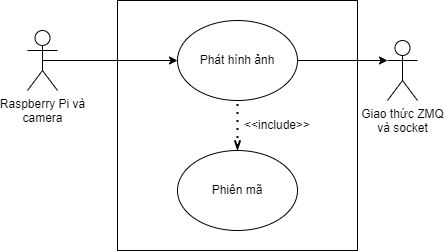
\includegraphics[width=0.8\textwidth]{publisher.png}
\label{pub_fig}
\caption{Biểu đồ ca sử dụng của publisher}
\end{figure}

\begin{table}[h]
    \centering
    \begin{tabular}{|p{0.2\linewidth}|p{0.7\linewidth}|}
    \hline
        Use case &  Phát hình ảnh\\
        \hline
        Actor &  Raspberry Pi và camera; socket và giao thức ZMQ\\ 
        \hline
        Brief Description &  Truyền tín hiệu ảnh đã mã hóa thông qua đường truyền socket thiết lập bới giao thức \O MQ. \\
        \hline
        Basic flow & \begin{enumerate}
            \item Tín hiệu ảnh được lấy về từ camera
            \item Ảnh được mã hóa thành chuỗi byte
            \item Chuỗi byte được gửi đi qua socket
        \end{enumerate}\\
        \hline
        Alternative flow &  Không có\\
        \hline
    \end{tabular}
    \caption{Đặc tả ca sử dụng của publisher}
    \label{table2}
\end{table}

\begin{table}[H]
    \centering
    \begin{tabular}{|p{0.2\linewidth}|p{0.7\linewidth}|}
    \hline
        Use case & Phiên mã \\
        \hline
        Actor & Thư viện PyCryptodome \\ 
        \hline
        Brief Description & Mã hóa ảnh bằng thuật toán AES-128 ECB\\
        \hline
        Basic flow & \begin{enumerate}
            \item Khởi tạo object mã hóa và key. Key sử dụng yếu tố thời gian để xoay vòng
            \item Gọi hàm encrypt để mã hóa
        \end{enumerate}\\
        \hline
        Alternative flow & Cập nhật lại khóa sau khoảng thời gian là 3600s\\
        \hline
    \end{tabular}
    \caption{Đặc tả ca sử dụng của phiên mã}
    \label{encode}
\end{table}

\begin{figure}[ht]
\centering
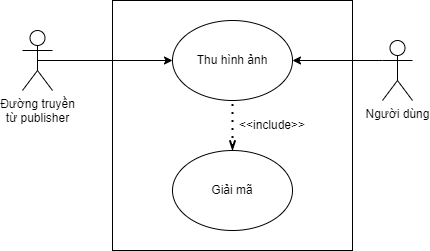
\includegraphics[width=0.8\textwidth]{subscriber.png}
\label{sub_fig}
\caption{Biểu đồ ca sử dụng của subscriber}
\end{figure}

\begin{table}[H]
    \centering
    \begin{tabular}{|p{0.2\linewidth}|p{0.7\linewidth}|}
    \hline
        Use case & Thu hình ảnh \\
        \hline
        Actor & Người sử dụng và đường truyền \\ 
        \hline
        Brief Description & Nhận tín hiệu ảnh đã mã hóa thông qua đường truyền socket thiết lập bới giao thức \O MQ.\\
        \hline
        Basic flow & \begin{enumerate}
            \item Chuỗi byte được nhận về từ publisher
            \item Chuỗi byte được giải mã và tái định dạng lại thành ảnh
            \item Ảnh được hiển thị trên giao diện.
        \end{enumerate} \\
        \hline
        Alternative flow &  Khi publisher đổi khóa, subscriber gửi exception để đồng bộ khóa theo thời gian \\
        \hline
    \end{tabular}
    \caption{Đặc tả ca sử dụng của subscriber}
    \label{table3}
\end{table}

\begin{table}[H]
    \centering
    \begin{tabular}{|p{0.2\linewidth}|p{0.7\linewidth}|}
    \hline
        Use case & Giải mã \\
        \hline
        Actor & Thư viện PyCryptodome \\ 
        \hline
        Brief Description & Giải mã chuỗi byte đại diện cho ảnh thành ảnh bằng thuật toán AES-128 ECB.\\
        \hline
        Basic flow & \begin{enumerate}
            \item Object AES được khởi tạo với khóa dựa vào thời gian
            \item Hàm AES.decrypt được gọi để giải mã
        \end{enumerate} \\
        \hline
        Alternative flow &  Nhận exception từ subscriber và đồng bộ khóa của object AES bằng yếu tố thời gian \\
        \hline
    \end{tabular}
    \caption{Đặc tả ca sử dụng của Giải mã}
    \label{decrypt}
\end{table}

\subsubsection{Lưu đồ thuật toán và giải thích}

\textbf{Publisher}

Hoạt động của publisher như sau:

Đầu tiên, publisher tạo ra 2 thread, một thread làm công việc mã hóa và truyền ảnh. Thread còn lại làm công việc đổi khóa.

Cơ chế đổi khóa của publisher phụ thuộc vào yếu tố thời gian. Mô hình Publisher - Subscriber không cho phép dữ liệu truyền từ Subscriber ngược về Publisher. Không những vậy, Publisher chỉ quan tâm đến việc truyền dữ liệu mà không cần biết các Subscriber có nhận được không. Chính vi vậy, ta cần có một cơ chế để đồng bộ khóa giữa Publisher và Subscriber.

Key để mã hóa được tạo bởi 14 ký tự, cộng với 2 ký tự để mô tả giờ. Theo cơ chế này, hệ thống sẽ có 24 khóa được xoay vòng trong một chu kỳ 24 giờ.

Với publisher, ta có biểu đồ sau đây:

\begin{figure}[H]
    \centering
    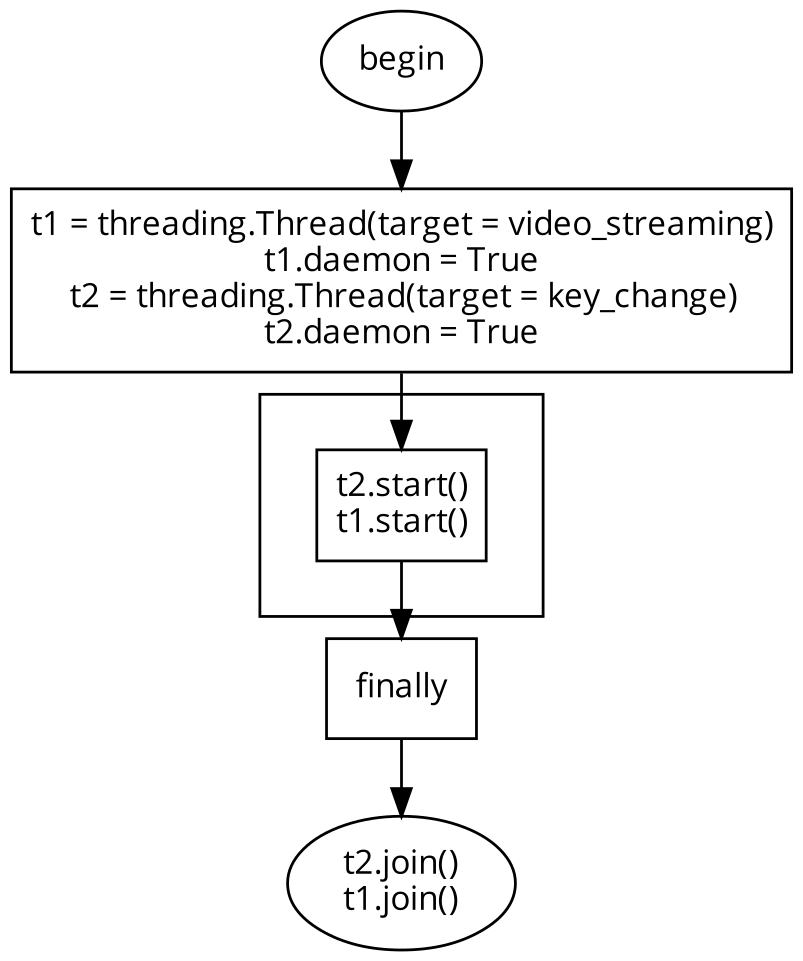
\includegraphics[width=0.6\linewidth]{pub_main_op.png}
    \caption{Lưu đồ thuật toán tổng quan của publisher}
    \label{fig:pub}
\end{figure}

Tổng quan hoạt động của hàm video\_streaming() là như sau:

Đầu tiên, tín hiệu ảnh được lấy từ stream của cảm biến ảnh Sunny P5V04A.

Ảnh được resize về độ phân giải 640x480, rồi được encode và byte hóa. Sau đó dữ liệu được pad lại và mã hóa bằng AES - 128, và được gửi qua socket thông qua giao thức \O MQ.

Khi gặp interrupt (thông qua việc nhấn Ctrl-C), chương trình sẽ dừng lại.

\begin{figure}[H]
    \centering
    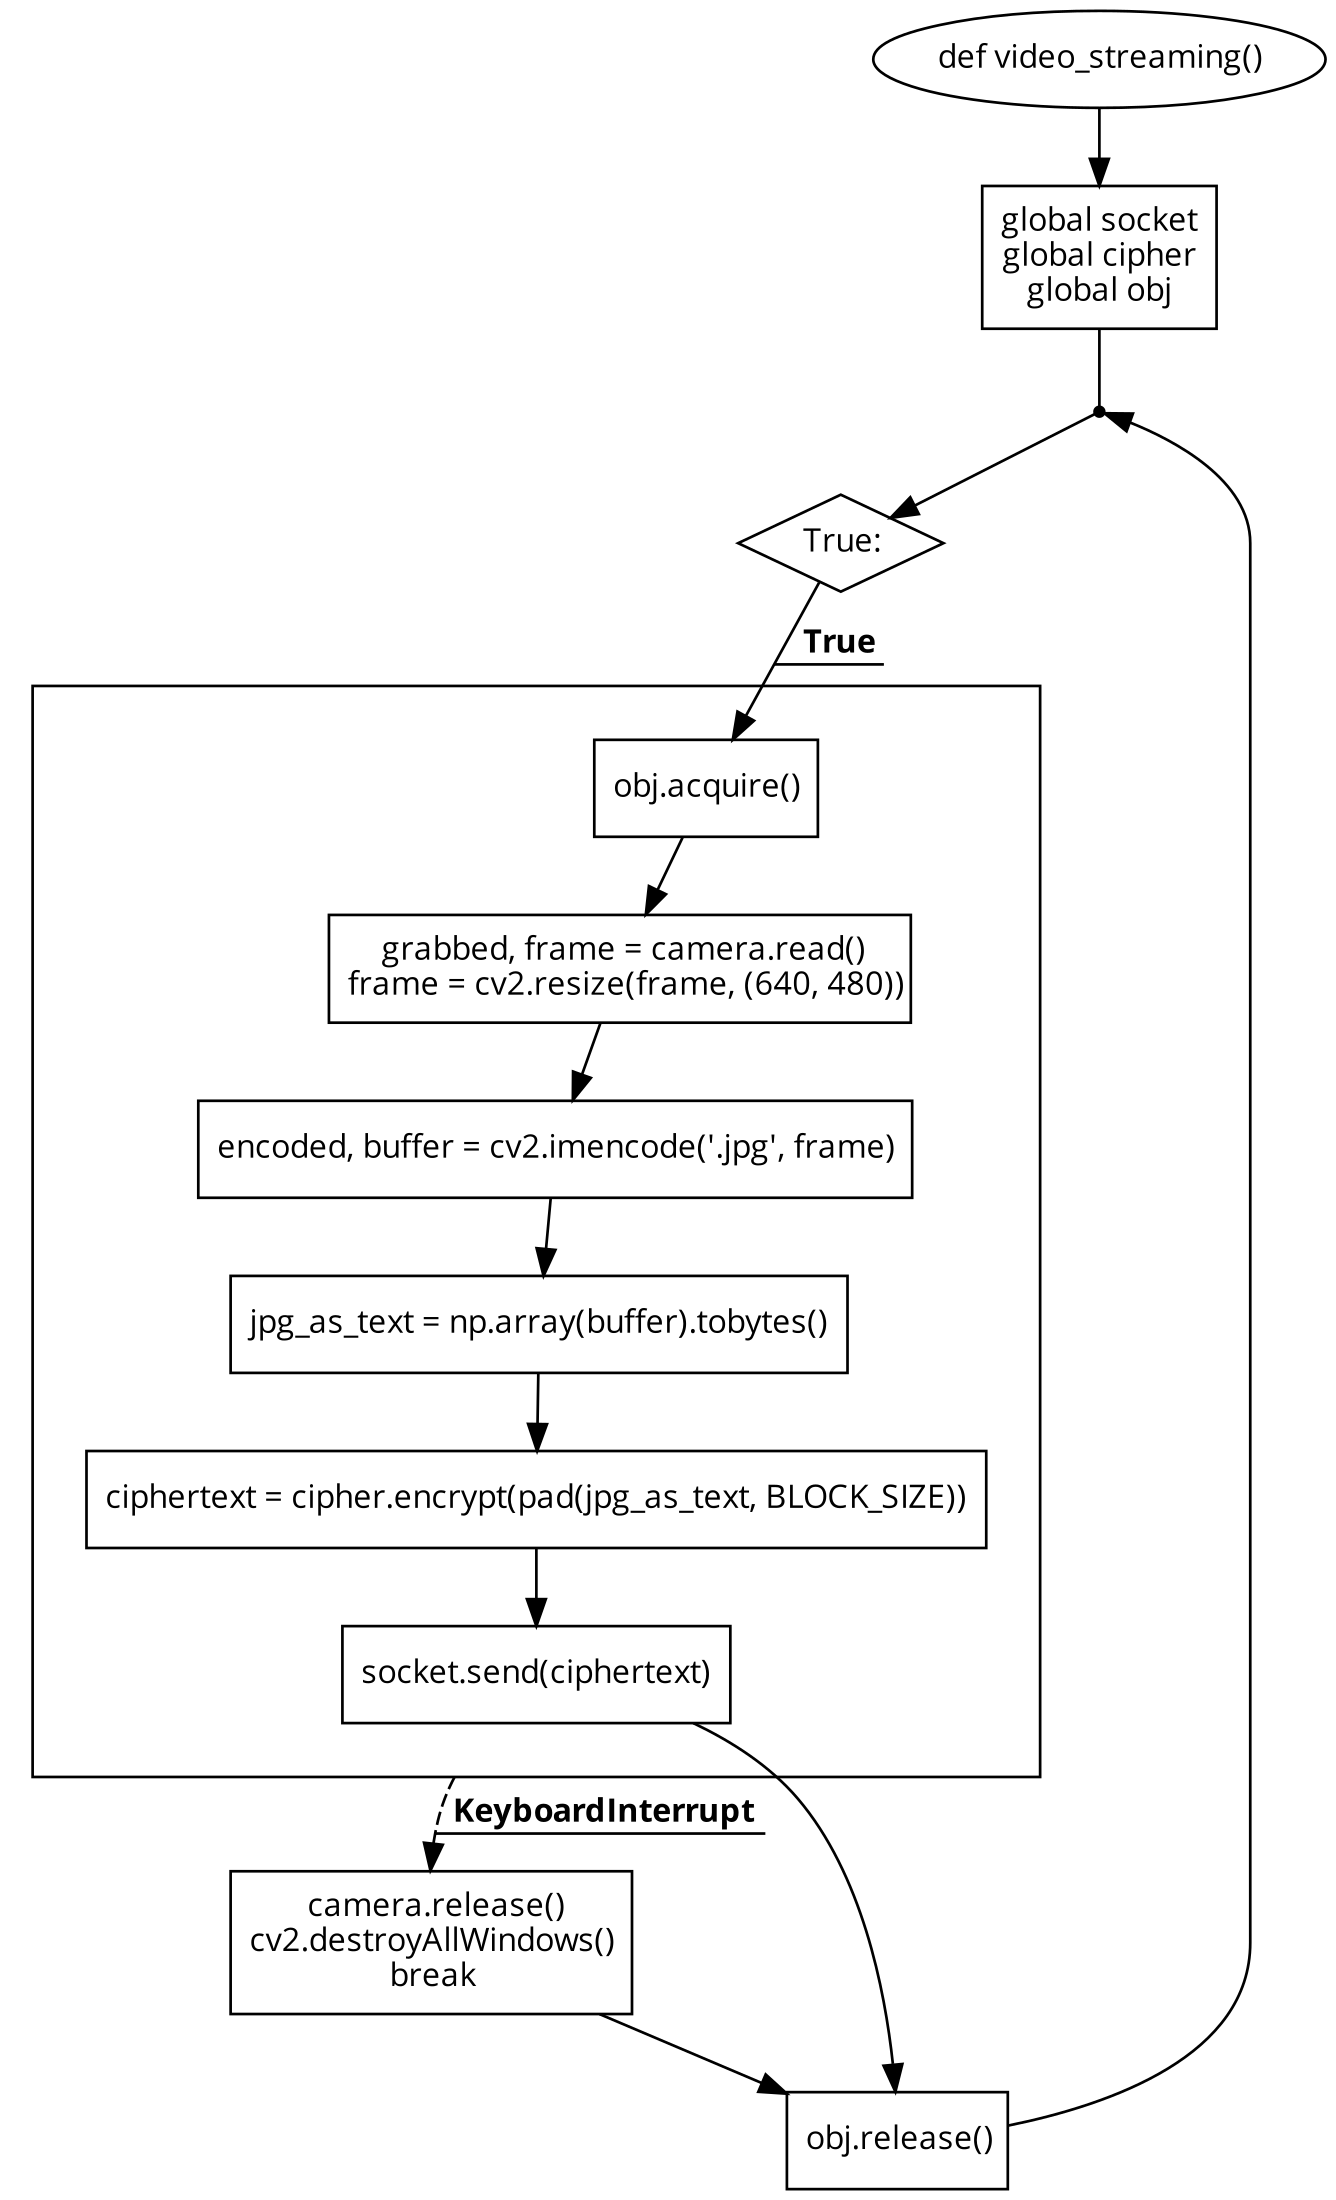
\includegraphics[width=0.6\linewidth]{video_streaming.png}
    \caption{Hàm video\_streaming()}
    \label{video_streaming}
\end{figure}

\break

\begin{figure}[H]
    \centering
    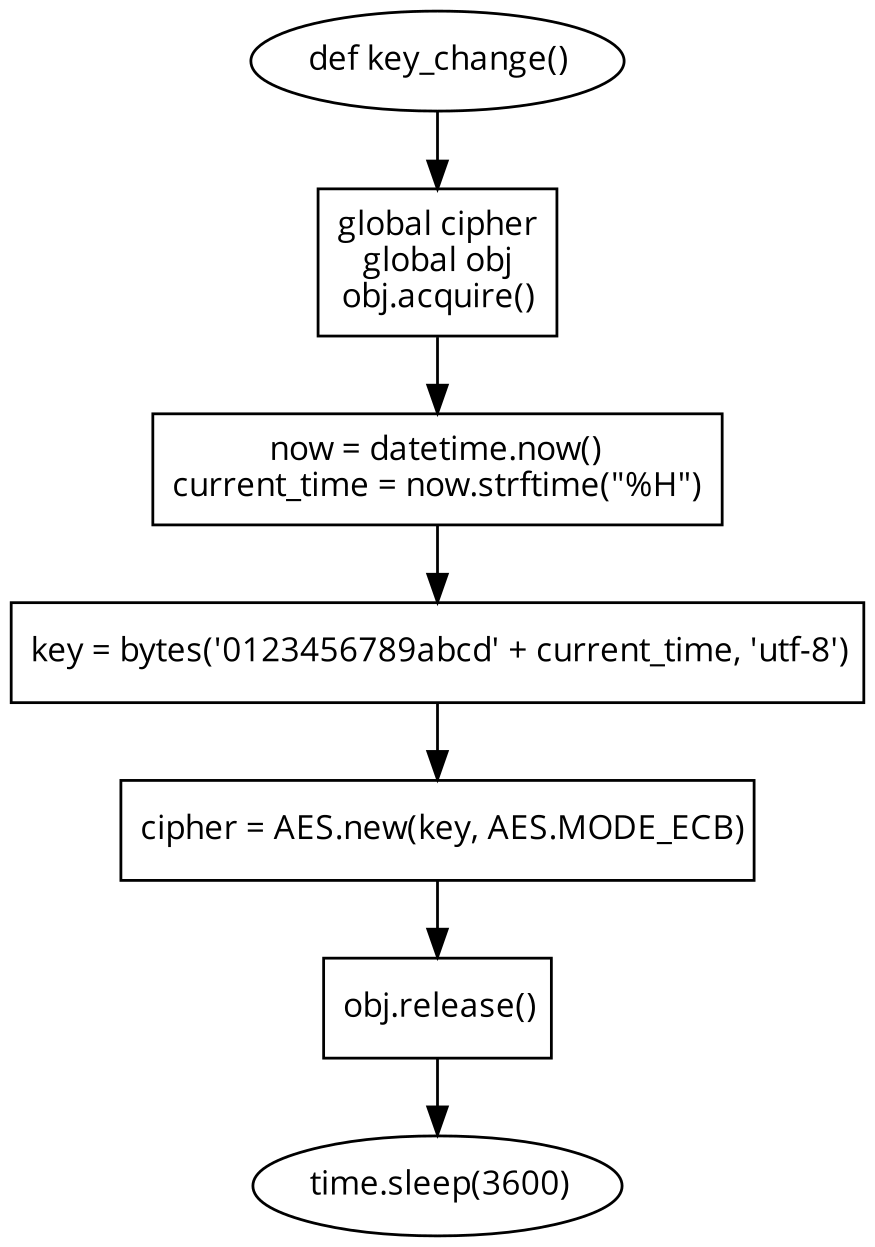
\includegraphics[width=0.6\linewidth]{key_change.png}
    \caption{Hàm key\_change()}
    \label{key_change}
\end{figure}

\textbf{Subscriber}

Quá trình đồng bộ khóa ở bên Subscriber được diễn ra như sau: Đầu tiên, khi khóa ở bên Publisher thay đổi, ngay lập tức chuỗi byte nhận được sẽ bị mất tương xứng và thư viện PyCryptodome sẽ ngay lập tức xuất ra một ValueError exception.

Lợi dụng exception này, ta bắt lấy exception thông qua một vòng try - except - finally. Trong except, ta sẽ lại sử dụng thời gian hệ thống để thay đổi khóa. Khi khóa được thay đổi thành công, dữ liệu trở thành tương xứng, và subscriber hoạt động lại bình thường 

Với subscriber, ta có biểu đồ sau đây:

\begin{figure}[H] 
    \centering
    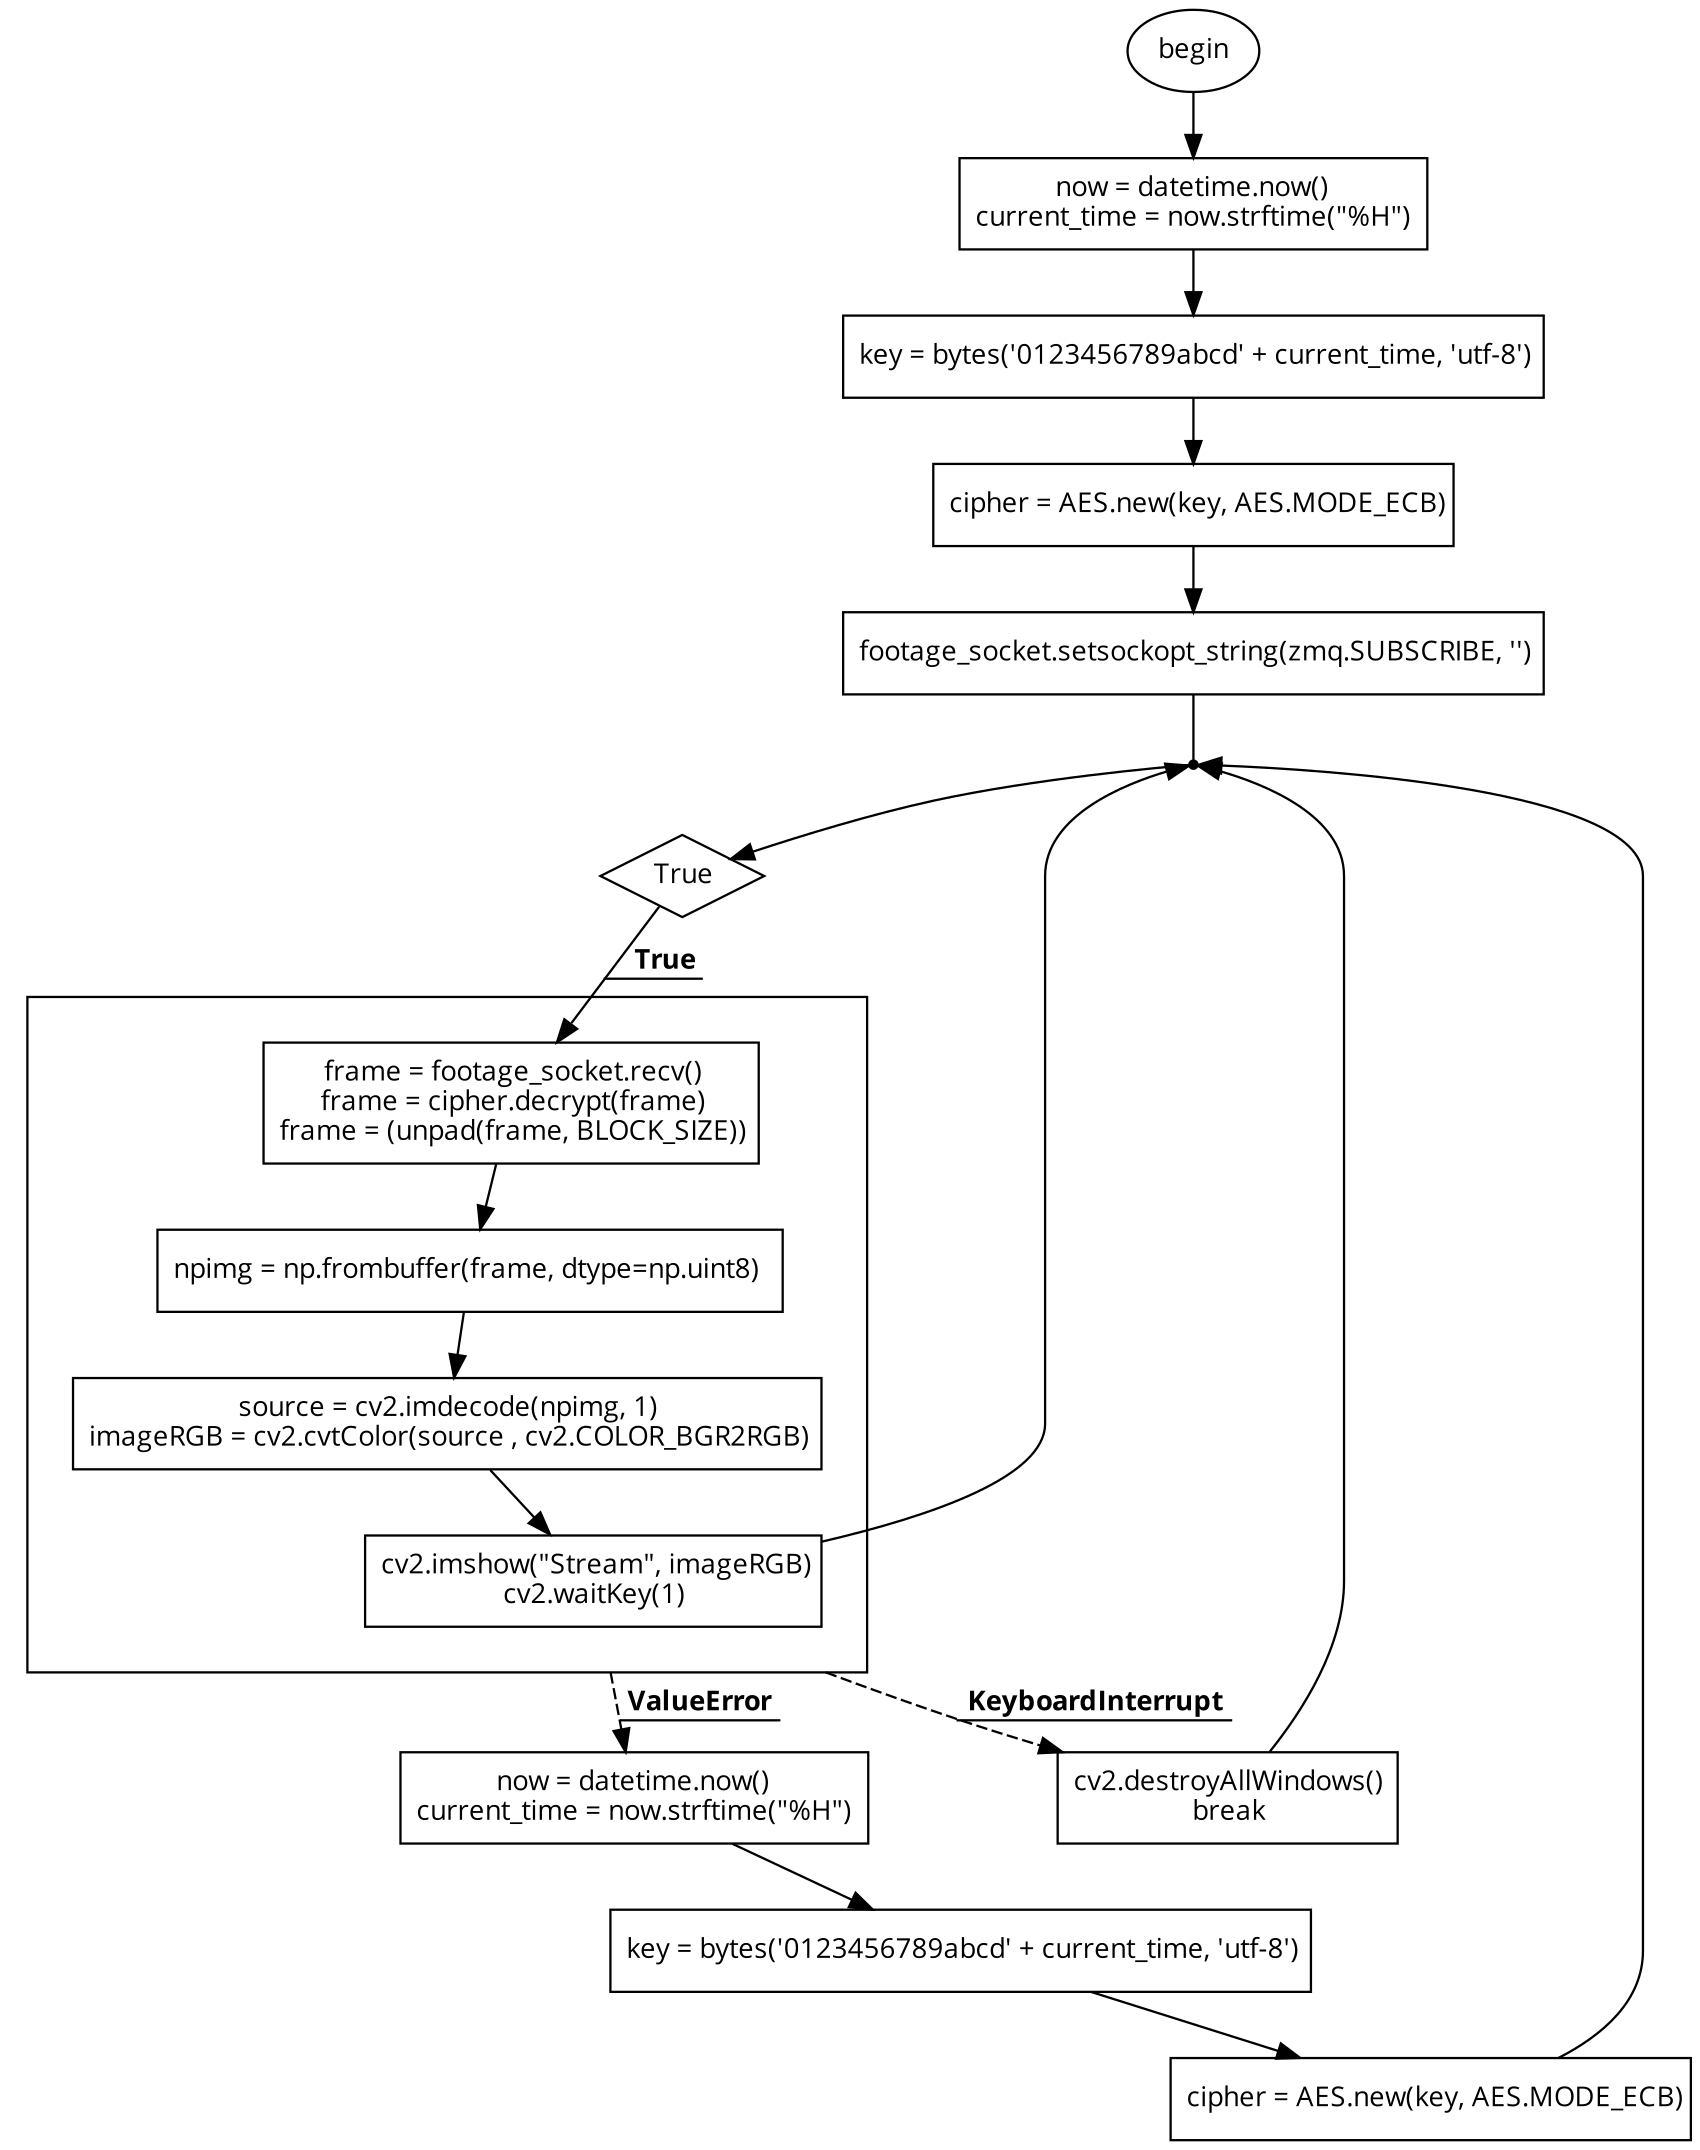
\includegraphics[width=0.8\textwidth]{sub_main_op.png}
    \caption{Lưu đồ thuật toán tổng quan của subscriber}
    \label{fig:sub}
\end{figure}

Quá trình giải mã và hiển thị ảnh được diễn ra như sau:

Trước hết, ảnh dưới dạng chuỗi byte được thu bởi subscriber. Sau đó, dữ liệu được giải mã bằng AES-128 và unpad. Tiếp đó, dữ liệu được tái định dạng từ dạng byte về dạng ma trận numpy với kích cỡ 3x640x480. Sau đó, ma trận được chuyển về dữ liệu dạng ảnh rồi được hiển thị.

\subsection{Thiết kế phần cứng}

\subsubsection{Sơ đồ làm việc}

Sơ đồ của hệ thống camera gồm 3 phần:
\begin{itemize}
    \item Các sensor: Cảm biến Sunny P5V04A.
    \item Bộ xử lý trung tâm: Raspberry Pi
    \item Các thiết bị subscriber.
    
\end{itemize}

\begin{figure}[H]
\centering
\begin{subfigure}[b]{0.4\textwidth}
\centering
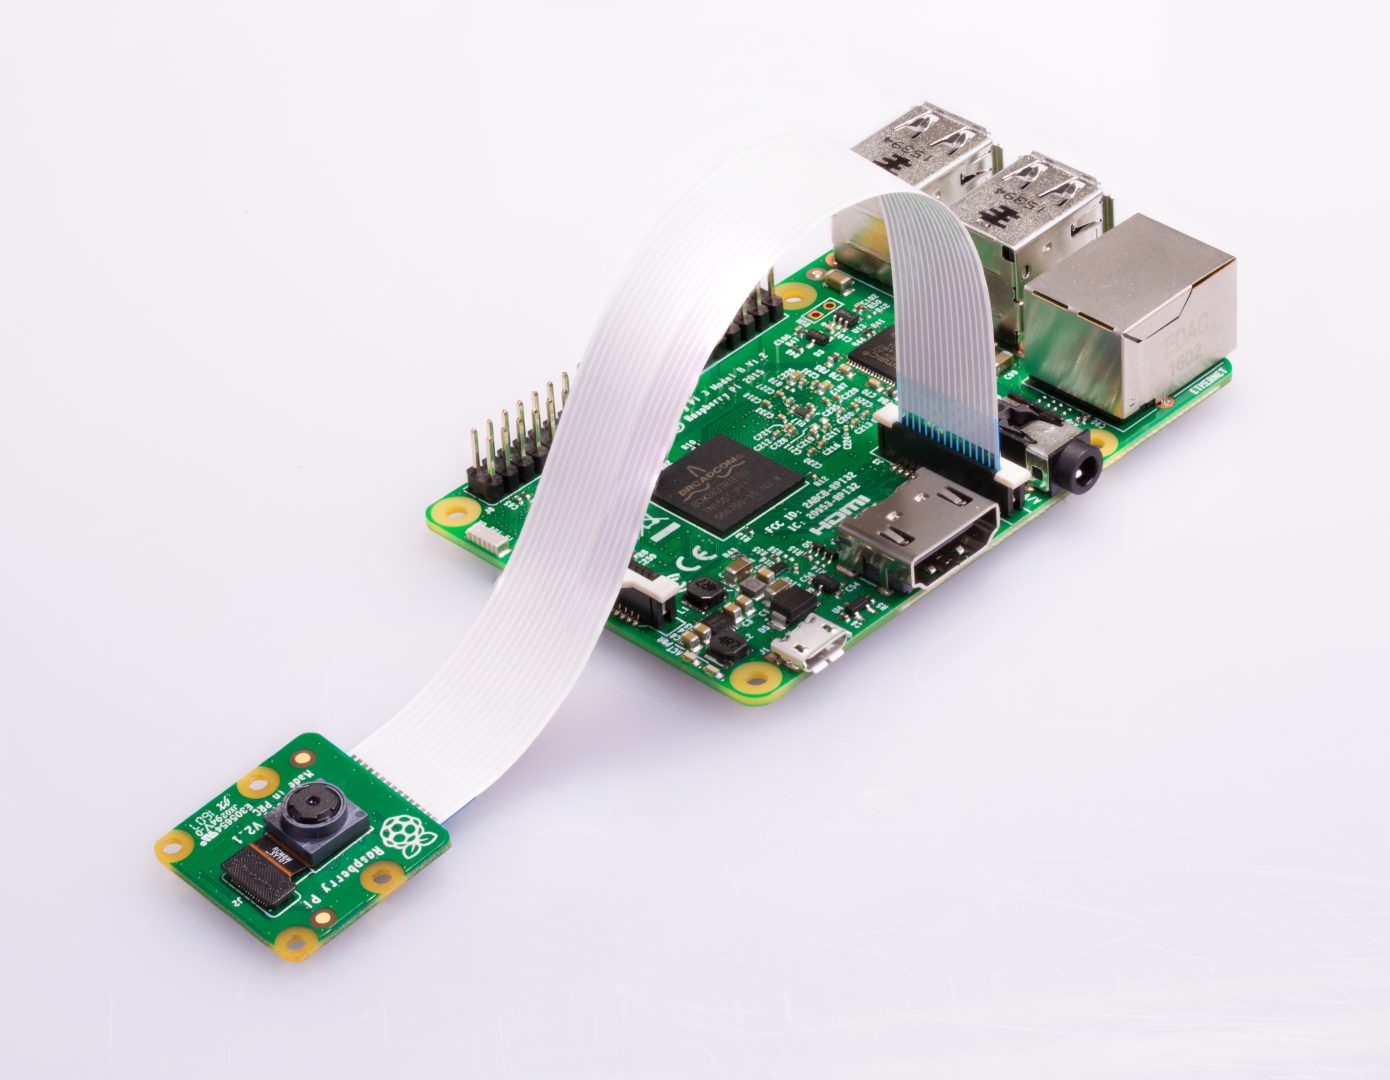
\includegraphics[width=\textwidth]{pi-camera-attached.jpg}
\caption{Ảnh minh họa publisher}
\label{pi_sys}
\end{subfigure}
\hfill
\begin{subfigure}[b]{0.4\textwidth}
\centering
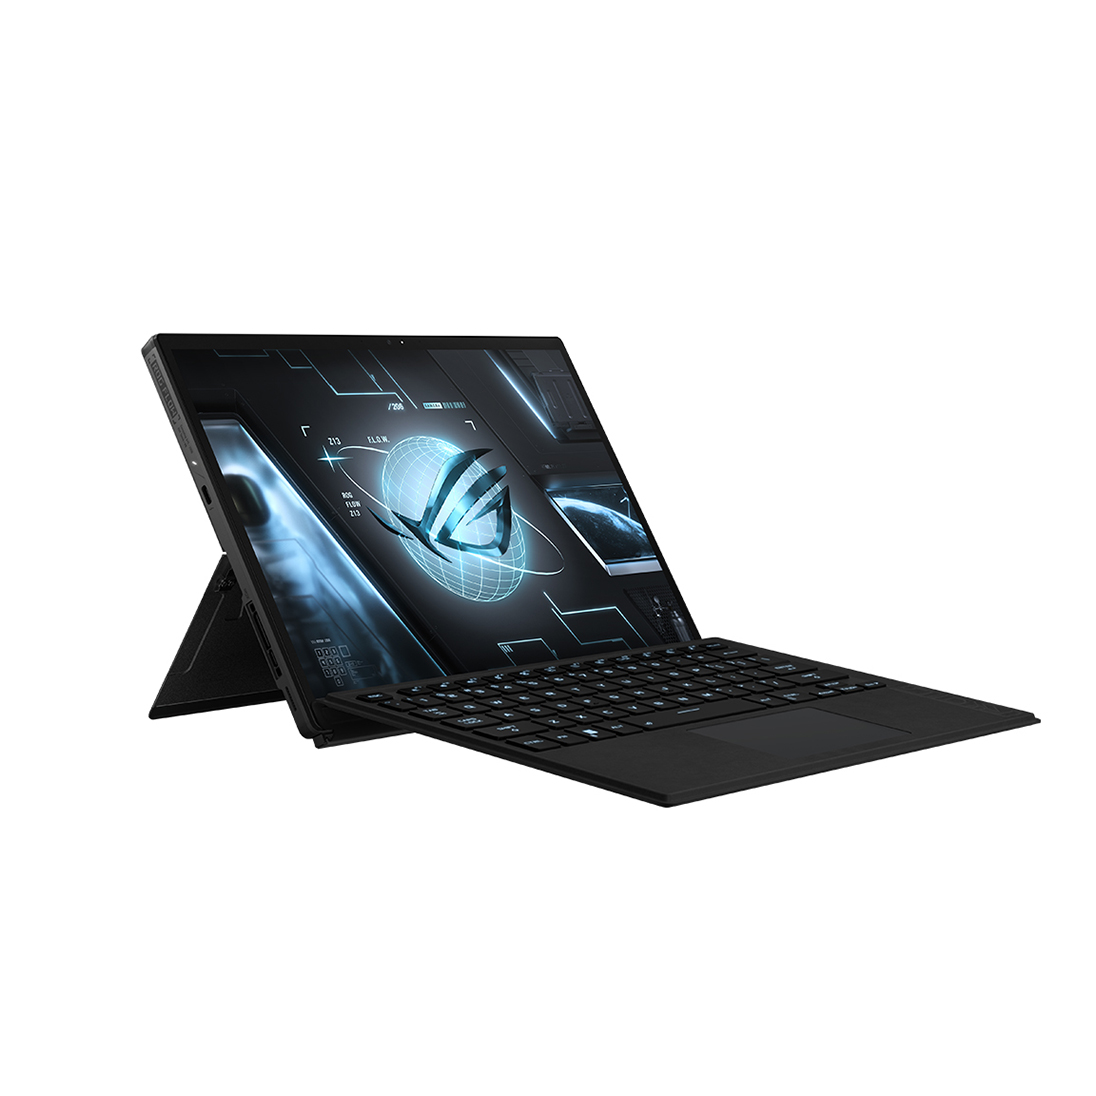
\includegraphics[width=\textwidth]{laptop.jpg}
    \caption{Ảnh minh họa subscriber}
    \label{laptop}
\end{subfigure}
\caption{Ảnh minh họa các thành phần của hệ thống camera}
\label{fig:three graphs}
\end{figure}

\subsection{Thử nghiệm}

\vfill

\begin{figure}[H]
    \centering
    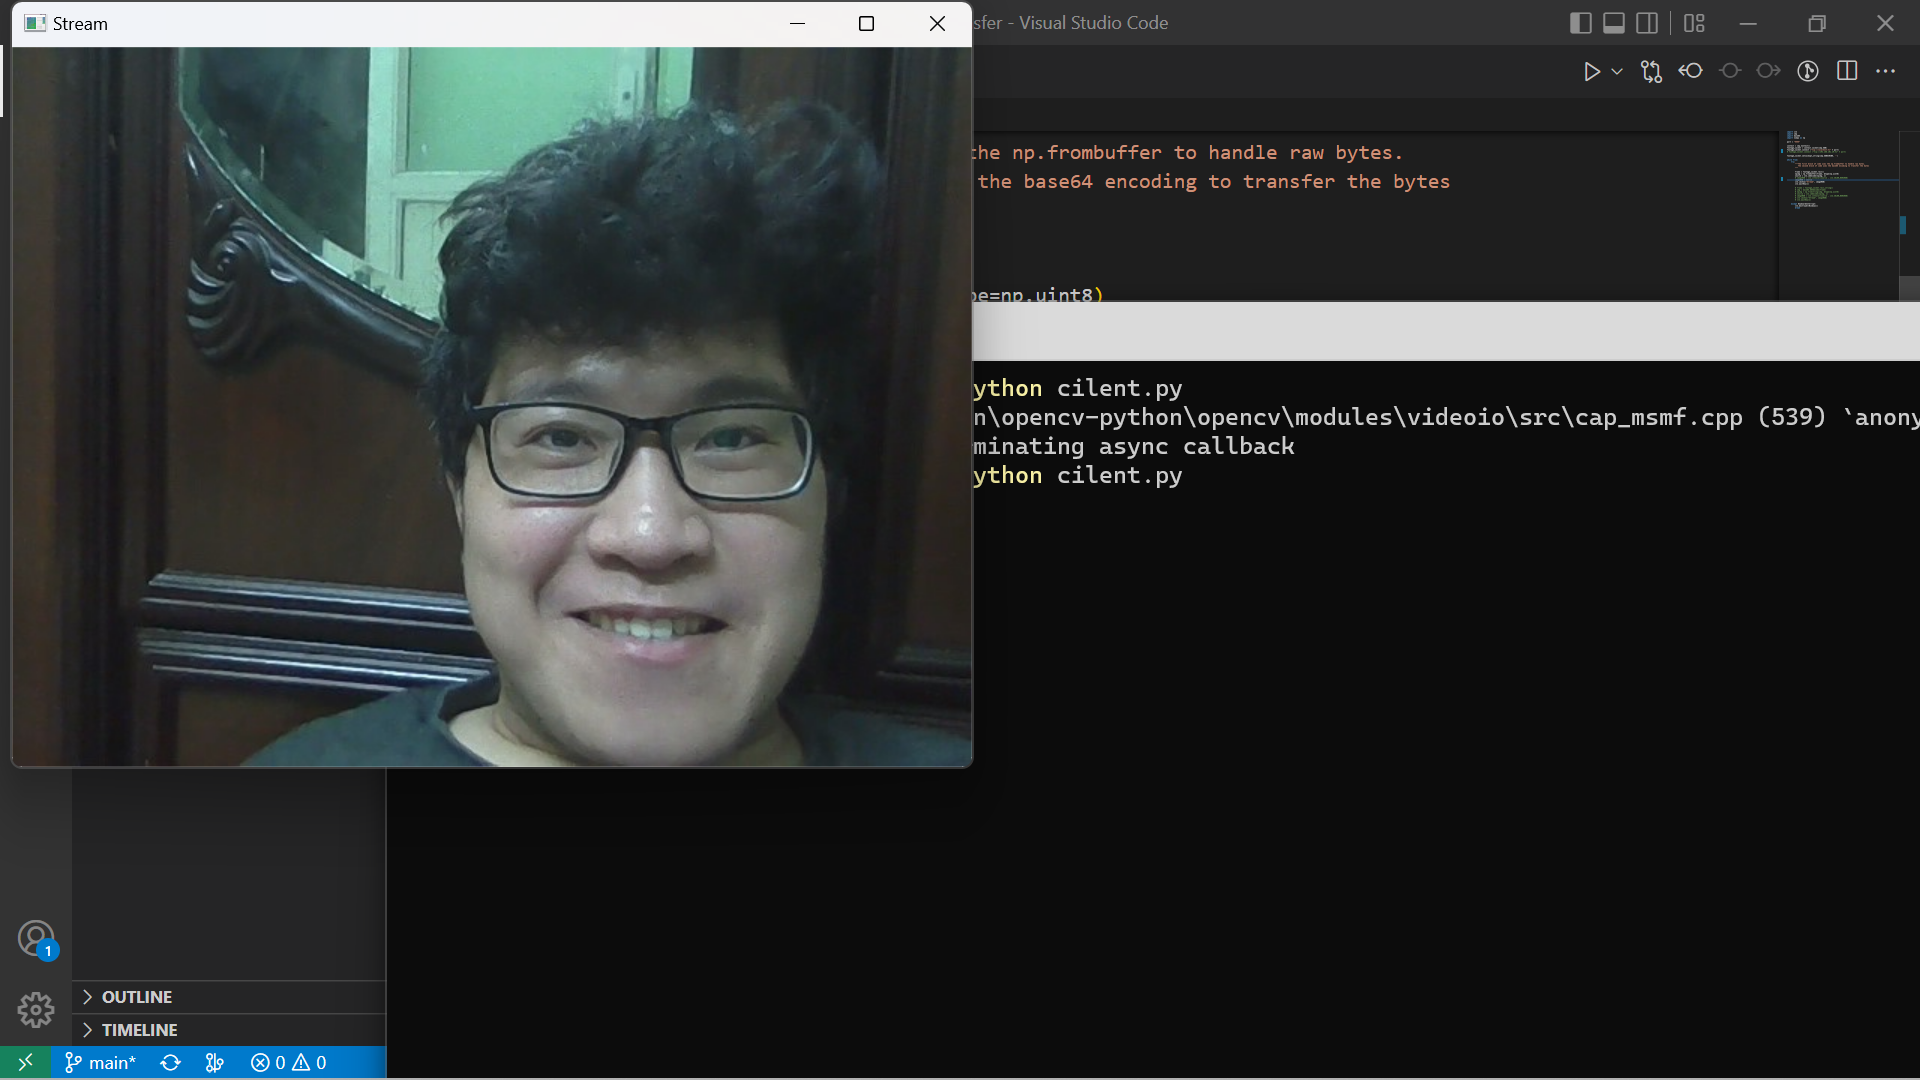
\includegraphics[width=0.8\textwidth]{demonstration.png}
    \caption{Minh họa mô hình camera}
    \label{demonstration}
\end{figure}

\vfill

\begin{figure}[H]
    \centering
    \includegraphics[width=0.8\textwidth]{2022-10-28.png}
    \caption{Minh họa tính chất Publisher - Subscriber của mô hình.}
    \label{demonstration2}
\end{figure}

\newpage

\section{Kết quả thực nghiệm}

\subsection{Kết quả thực hiện đề tài}
Qua việc thực hiện đồ án về bảo mật trong hệ thống camera giám sát, em đã tích lũy được thêm nhiều kiến thức về sử dụng các tính năng của Raspberry Pi, sensor camera Sunny P5V04A,…

\subsection{Nhận xét và đánh giá}

Sau thời gian tìm hiểu, thiết kế và thi công đồ án với đề tài “Bảo mật video truyền trên mạng WiFi sử dụng Raspberry Pi và giao thức ZeroMQ” đã và đang hoàn thiện.

Mô hình hệ thống hoạt động tương đối ổn định, có thể làm việc liên tục, đạt được yêu cầu ban đầu đề ra.

Độ ổn định của máy phụ thuộc vào nguồn điện cung cấp.

Do hạn chế về kiến thức cũng như thời gian, nguồn tham khảo chủ yếu là thông qua mạng internet nên đề tài còn có hạn chế:

\begin{itemize}
\item Tính thực tiễn chưa cao do giá thành Raspberry Pi 3 B+ rất cao.
\item Tính thẩm mỹ của máy chưa cao.
\end{itemize}
\subsection{Phương hướng phát triển đề tài}
Do đề tài mới chỉ dừng lại ở việc thiết kế mô hình thí nghiệm với quy mô nhỏ nên giá thành để sản xuất ra một sản phẩm chưa ổn định. vì vậy để có thể phát triển sản phẩm hơn trong đời sống, em xin đề xuất một vài phương án để cải thiện đề tài:
\begin{itemize}
\item Sản xuất số lượng nhiều để giảm giá thành sản phẩm.
\item Mở rộng Raspberry Pi thành bộ điều khiển cho nhà thông minh, mở rộng hệ thống camera giám sát
\item Sử dụng nguồn dự phòng cho hệ thống 
\end{itemize}
\subsection{Kết luận}
Sau thời gian học tập và tìm hiểu để thực hiện theo tiến độ, đề tài đã hoàn thành theo đúng mục tiêu đã đề ra.

Em xin chân thành cảm ơn sự hướng dẫn, giúp đỡ các thầy cô, bạn bè để nhóm hoàn thành nội dung đề tài theo đúng mục tiêu và tiến độ đặt ra.

Dù đã rất cố gắng, nhưng do thời gian có hạn và bước đầu thực hiện nghiên cứu, nên đề tài không tránh khỏi thiếu sót, mong nhận được sự góp ý của các thầy cô, bạn bè.

\newpage

\appendix

\section{Mã nguồn bài tập lớn}

publisher.py
\begin{lstlisting}[language=Python]
import base64
import threading
import cv2
from sklearn.neighbors import KernelDensity
import zmq
import time
import numpy as np
from datetime import datetime
from Crypto.Util.Padding import pad, unpad
from Crypto.Cipher import AES
BLOCK_SIZE = 32
port = "5555"

context = zmq.Context()
socket = context.socket(zmq.PUB)
socket.bind("tcp://*:%s" % port) # binds to anything that wants to connect

now = datetime.now()
current_time = now.strftime("%H")
key = bytes('0123456789abcd' + current_time, 'utf-8')

cipher = AES.new(key, AES.MODE_ECB)
camera = cv2.VideoCapture(0)  # init the camera
obj = threading.Semaphore()

def video_streaming():
    global socket
    global cipher
    global obj
    while True:
        try:
            obj.acquire()
            grabbed, frame = camera.read()  # grab the current frame
            frame = cv2.resize(frame, (640, 480))  # resize the frame
            encoded, buffer = cv2.imencode('.jpg', frame)
            jpg_as_text = np.array(buffer).tobytes()
            ciphertext = cipher.encrypt(pad(jpg_as_text, BLOCK_SIZE))
            socket.send(ciphertext)

        except KeyboardInterrupt:
            camera.release()
            cv2.destroyAllWindows()
            break

        finally:
            obj.release()

def key_change():
    global cipher
    global obj
    obj.acquire()
    now = datetime.now()
    current_time = now.strftime("%H")
    key = bytes('0123456789abcd' + current_time, 'utf-8')
    cipher = AES.new(key, AES.MODE_ECB)
    obj.release()
    time.sleep(3600)

t1 = threading.Thread(target = video_streaming)
t1.daemon = True # Kill thread when main program ends
t2 = threading.Thread(target = key_change)
t2.daemon = True

try:
    t2.start()
    t1.start()
finally:
    t2.join()
    t1.join()

\end{lstlisting}

subscriber.py
\begin{lstlisting}[language=Python]
import cv2
from datetime import datetime
import zmq
import base64
import numpy as np
from Crypto.Util.Padding import pad, unpad
from Crypto.Cipher import AES
BLOCK_SIZE = 32
port = "5555"

context = zmq.Context()
footage_socket = context.socket(zmq.SUB)
footage_socket.connect ("tcp://localhost:%s" % port)
# footage_socket.connect ("tcp://raspberrypi.local:%s" % port)
now = datetime.now()
current_time = now.strftime("%H")
key = bytes('0123456789abcd' + current_time, 'utf-8')
cipher = AES.new(key, AES.MODE_ECB)
footage_socket.setsockopt_string(zmq.SUBSCRIBE, '')

while True:
    try:
        frame = footage_socket.recv()
        frame = cipher.decrypt(frame)
        frame = (unpad(frame, BLOCK_SIZE))
        npimg = np.frombuffer(frame, dtype=np.uint8)
        source = cv2.imdecode(npimg, 1)
        # imageRGB = source
        imageRGB = cv2.cvtColor(source , cv2.COLOR_BGR2RGB)
        cv2.imshow("Stream", imageRGB)
        cv2.waitKey(1)

    except KeyboardInterrupt:
        cv2.destroyAllWindows()
        break

    except ValueError:
        now = datetime.now()
        current_time = now.strftime("%H")
        key = bytes('0123456789abcd' + current_time, 'utf-8')
        cipher = AES.new(key, AES.MODE_ECB)
    
\end{lstlisting}

\newpage

\section{Tài liệu tham khảo}

[1] Thư viện OpenCV - https://docs.opencv.org/4.x/

[2] Thư viện \O MQ - https://zeromq.org/get-started/?language=python\&library=pyzmq

[3] Thư viện PyCryptodome - https://pycryptodome.readthedocs.io/en/latest/src/cipher/aes.html

[4] Thư viện Numpy - https://numpy.org/doc/stable/

[5] Adrian Rosebrock - Live video streaming over network with OpenCV and ImageZMQ (2019)

[6] Andrew Laughlin - The cheap security cameras inviting hackers into your home (2019)

\end{document}